\begin{introduction}
    \item 基本概念
\end{introduction}

\section{基本概念}
    \subsection{原子单位制}
        在量子化学计算中,由于计算机的数值模拟只具有有限的精度,因此方程的系数往往会很大的影响到结果的准确性,为了最大限度地除去这类干扰,我们常常使用原子单位制来简化式子的表达。相比于一般的量子化学书对原子单位制的说明,我希望用稍微严谨一点的表述说明原子单位制的选取\footnote{本节内容主要参考了小时百科以及wiki有关Hartree atomic units的说明}。
        
        原子单位制的目的就是将方程去量纲化。首先考虑一个相对简单的粒子来引出大致的思路。考虑一维的含时Schrodinger方程:
        \begin{equation}
            -\frac{\hbar^2}{2m}\frac{\partial^2\Psi}{\partial x^2}+V\Psi=i\hbar \frac{\partial \Psi}{\partial t}
        \end{equation}
        
        我们将上式所有的物理量转换为无量纲的量,即:$x=x_a\beta_x,m=m_a\beta_m,V=V_a\beta_V,\psi=\psi_a\beta_{\psi},t=t_a\beta_t$,其中诸如$x_a,m_a$之类的量都是没有量纲的。代入上式并化简即可以得到:
        \begin{equation}
            -\Big(\frac{\hbar^2}{\beta_m\beta_x^2\beta_E}\Big)\frac{1}{2m_a}\frac{\partial^2\psi_a}{\partial x_a^2}+V_a\psi_a=i\Big(\frac{\hbar}{\beta_t\beta_E}\Big)\frac{\partial\psi_a}{\partial t_a}
        \end{equation}
        
        唯一可能含有量纲的数就是$\frac{\hbar^2}{\beta_m\beta_x^2\beta_V},\frac{\hbar}{\beta_t\beta_V}$。为了得到不含有量纲的方程,我们人为地令这两个量为1,即:
        \begin{align}\label{equ12:restrictA}
            \begin{split}
                \frac{\hbar^2}{\beta_m\beta_x^2\beta_E}=&1\\
                \frac{\hbar}{\beta_t\beta_E}=&1
            \end{split}
        \end{align}
        
        同时考虑波函数地归一,我们可以得到另一个无量纲组合量:
        \begin{align}\label{equ12:restrictB}
                1=\int |\Psi|^2dx=(\beta_{\psi})^2\beta_x\int \psi^2_adx_a=(\beta_{\psi})^2\beta_x
        \end{align}
        
        特别的,对于N维波函数,我们可以很容易地推广得到:
        \begin{equation}
            (\beta_{\psi})^2\beta_x^N=1
        \end{equation}
        
        由\ref{equ12:restrictA},\ref{equ12:restrictB}式,我们可以知道上述量的自由度为2(比如说知道了$\beta_x,\beta_m$,我们就可以推出其它所有的量)。一般来说,我们令$\beta_m$为电子的质量,$\beta_x$为Bohr半径,于是我们可以得到其它量的取值:
       \begin{align}
           \begin{split}
               \beta_E=&\frac{\hbar^2}{m_ea_0^2}\\
               \beta_t=&\frac{m_ea_0^2}{\hbar}
           \end{split}
       \end{align}
       
       我们称$\beta_E$的单位为Hartree。简单来说,我们可以认为原子单位制就是将$\hbar,a_0.e,m_e$四个量变为1,上述四个量分别表示原子单位制下的运动,长度,电荷和质量量度。基于上面的“定义”,我们就可以将具有M个核子和N个电子的波函数的Hamiltonian写成如下简单的形式:
       \begin{equation}
           \hat{H}=-\sum_{A=1}^M\frac{1}{2M_A}\nabla^2_A-\sum_{i=1}^N\frac{1}{2}\nabla_i^2+\sum_{A=1}^{M}\sum_{B>A}^M\frac{Z_AZ_B}{R_{AB}}+\sum_{i=1}^{N}\sum_{j>i}^N\frac{1}{r_{ij}}-\sum_{i=1}^N\sum_{A=1}^M\frac{Z_A}{r_{iA}}
       \end{equation}
       
       式中,$A,B$是核的标号,$i,j$是电子的标号,$Z_A,Z_B$为核子的标号。上述五项分别表示核的动能,电子的动能,核之间的相互作用,电子之间的相互作用,核与电子之间的相互作用。
    \subsection{B-O近似}
        由上节的讨论,虽然我们已经写出了一般具有M个核子,N个电子的体系Hamiltonian的表达式,由此我们可以写出多电子体系对应的定态方程:
        \begin{equation}\label{equ12:multiele_stationaryA}
            \hat{H}\psi(q_i,Q_j)=E\psi(q_i,Q_j)
        \end{equation}
        
        其中$q_i$是电子的广义坐标;$Q_j$是核的广义坐标。虽然定态方程的形式看上去非常简单,但是实际上这个体系是一个多体问题,不能精确求解,因此我们需要发展各种合理的近似手段去化简方程。这其中最基本最简单但是较为精确的假设就是Born-Oppenheimer近似。
        \subsubsection{定核假设}
        B-O近似的本质在于分离核与电子的运动,这个想法的出发点在于核子与质子的质量差别很大(即$m_n>>m_e$),因此可以知道核子的运动是比电子慢很多的。于是对于原子核的每一次微小运动,我们可以认为电子总是能够迅速地跟上核的运动并迅速适应新的势场(即电子对核运动的响应是瞬时的\footnote{简单来说,相对于电子的运动,我们可以忽略核的运动})。于是我们自然可以假设原子核处在空间任意一个相对位置时,分子的电子状态和原子核一直固定在空间某一点对应的分子的电子状态相等。这也表明电子总是在固定的核势场中运动,从而对于\ref{equ12:multiele_stationaryA}式的定态方程的Hamiltonian,如果我们只考虑电子的运动,此时我们可以忽略核的动能项,得到电子运动的定态方程:
        \begin{equation}
            (\hat{H_{el}})\psi_{el}=E^{el}\psi_{el}
        \end{equation}
        
        其中:
        \begin{align}\label{equ12:multiele_stationaryB}
                \hat{H_{el}}=-\sum_{i=1}^N\frac{1}{2}\nabla_i^2+\sum_{i=1}^{N}\sum_{j>i}^N\frac{1}{r_{ij}}-\sum_{i=1}^N\sum_{A=1}^M\frac{Z_A}{r_{iA}}+\sum_{A=1}^{M}\sum_{B>A}^M\frac{Z_AZ_B}{R_{AB}}
        \end{align}
        
        其中$E^{el}$是包含了核子之间相互作用的电子能量,对于一般我们的讨论来说,$R_{AB}$是一个不随电子坐标改变的常数,但是势能的大小却与核的构型(configuration)有关,因此我们可以明确\ref{equ12:multiele_stationaryB}式的函数形式:
        \begin{align}
            \begin{split}
                \psi_{el}=&\psi_{el}(q_i,Q_j)\\
                E^{el}=&E^{el}(Q_j)
            \end{split}
        \end{align}
        
        其中$q_\alpha$是参数(parameter),$q_i$是变量(variable)。
        \subsubsection{绝热近似}
        假设电子的Schrodinger方程已经被完全求解,下面我们讨论核运动。根据上面的讨论,由于电子对核运动的响应是瞬时的,因此当核进行移动时,我们可以忽略电子运动的影响。换而言之,核的运动是核的构型的函数,我们可以将电子看作连接核的弹簧,因此核运动产生的势场应该包含了核的相互作用以及电子对核产生的势场,即$E^{el}(Q_j)$;同时考虑其动能,因此我们可以写出核运动的定态方程:
        \begin{align}
            \begin{split}
                \hat{H_N}\psi_N(Q_j)=E\psi_N(Q_j)
            \end{split}
        \end{align}
        
        其中\footnote{该式的$j$是一个常数,不是一个变化的值,代表核受到电子的某种势场作用}:
        \begin{equation}
            \hat{H_N}=-\sum_{A=1}^M\frac{1}{2M_A}\nabla^2_A+E^{el}(Q_j)
        \end{equation}
        
        $E$和\ref{equ12:multiele_stationaryA}式中的$E$一样,代表体系的总能量,是一个常数。上述论述统称为绝热近似(adiabatic approximation)。Born和Fork对绝热近似的定义是\footnote{wiki上的原文为:A physical system remains in its instantaneous eigenstate if a given perturbation is acting on it slowly enough and if there is a gap between the eigenvalue and the rest of the Hamiltonian's spectrum}:一个物理系统保持在它的瞬时本征态,如果给定的扰动作用在它上的速度足够慢,并且在本征值和哈密顿谱的其余部分之间有一个间隙。可以看到,这里的绝热与热力学的绝热\footnote{热力学中的绝热指体系不与环境发生热量和物质的交换}不同,反倒和准静态过程的定义类似,我的理解为\footnote{这里的理解基于wiki的词条,词条的原文为:Gradually changing conditions allow the system to adapt its configuration, hence the probability density is modified by the process. If the system starts in an eigenstate of the initial Hamiltonian, it will end in the corresponding eigenstate of the final Hamiltonian.}:体系运动的每一步由于弛豫\footnote{所谓弛豫涉及到两个时间:"内部"时间$T_i$,代表体系自身运动;"外部"运动$T_e$,代表环境参数变化的时间。弛豫就是这两个时间的博弈,显然,绝热近似要求$T_e>>T_i$}较大(有点像平衡态的感觉),因此当核从$Q_j$移动到$Q_{j'}$时,我们可以认为电子没有受到核运动的扰动发生电子的跃迁,此时势能函数永远都是$Q_j$的函数,如此,系统的每一个状态都是构型的函数。
        
        \begin{remark}
        这里有两个例子帮助您更好的理解绝热近似的思想\footnote{这两个绝好的例子可以在wiki和Griffiths的CH7中找到}:第一个例子是无阻尼单摆在一个箱子里摆动。试想,如果我拿着箱子猛烈地移动它,那么单摆一定会混乱的移动;而如果我缓慢的移动这个箱子,那么单摆仍然会相对于箱子做振幅一样的往复摆动。
        \begin{figure}[H]
            \centering
            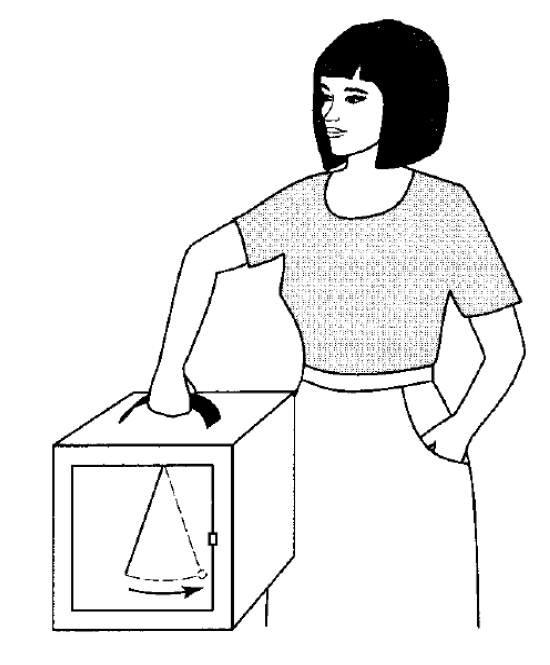
\includegraphics[width=0.5\textwidth]{figure/adiabaticprocess.png}
            \caption{如果箱子移动得非常缓慢,里面的摆将在与原来平面平行的平面振动,振幅保持不变}
            \label{fig:adiabaticprocess}
        \end{figure}
        
        根据这个例子启发,我们可以将核看作我们提的箱子,而将电子看作往复运动的单摆。由于核的运动相比电子来说很慢,因此核无论处于什么位置,我们都能得到电子的能量。换句话说,电子的能量$E^{el}$是以核的坐标位参数的(即$E^{el}(Q_1,Q_2,\dots,Q_m)$),我们称此时的电子能量构成势能面(potential energy surface)
        
        这个例子是对绝热运动的形象理解。分析这类问题,一般来说先把外部参数设为常量,在求解到最后的时候再允许外部参数随时间变化。一个经典的例子\footnote{这个方法在定核近似中其实已经分析过了}是氢原子离子的求解,我们先假设原子核质心距离为R,然后求解电子的运动。如果我们求解出了能量,再令R是能量的函数,从而可以得到平衡位置和原子核振动的频率。这种先固定原子核位置(可以理解为变量参数化),再求解电子运动,最后利用电子运动的信息得到核运动的信息就是B-O近似的核心思想。
        \end{remark}
        
        我们下面较为严格的证明绝热近似。
        
        
        定核近似与绝热近似合在一起称为B-O近似。可以发现,在该近似下,多电子体系的Hamiltonian被分解为了核运动算符$\hat{H_N}$与电子运动算符$\hat{H_{el}}$的直和。因此方程的解可以写成核运动波函数与电子运动波函数的直接乘积:
        \begin{equation}
            \psi(q_i,q_\alpha)=\psi_N(q_\alpha)\psi_{el}(q_i,q_\alpha)
        \end{equation}
        
        在量子化学的学习中,我们往往更为重视电子的运动,因为它决定着物质的化学性质。